\chapter{行人导航系统设计}
	
\section{系统设计目标与需求分析}
	
本行人导航系统设计目的是城市环境的行人导航,以智能的技术手段,为行人提供绕行障碍物、快速到达目标的路径规划,因此本行走式行人导航系统需满足以下要求:基于用户的起终点坐标信息,规划最短路径,包括:考虑道路距离、行人速度、路况、交通规则;实时感知、规避障碍物(包括其他行人、交通事故、施工工地等)、实时监控周边环境信息并调整路径、应对突发障碍物或路径更改;实时感知周边环境并调整路径和决策。

系统主要目标是构建一个可训练、可测试、可交互的行人导航平台,需在复杂动态环境中提供快速、精确、安全的行人导航服务,而这些也是如今虚拟人发展所需要的一个重要技术,可以分为功能需求和非功能需求。

\textbf{功能需求}:包括方向控制、速度控制、行走状态切换的真实感行人运动控制;路径规划、躲避障碍任务的学习环境搭建;基于激光雷达和碰撞探测器对动态障碍物进行感知与反馈;图形界面参数设置与训练进程控制。

\textbf{非功能需求}:系统应支持在Carla仿真平台运行并具备高鲁棒性与低资源消耗,强化学习训练过程需保持稳定并具备扩展能力,用户交互界面需具有人机交互性强与操作简洁的特点。

\section{系统结构设计}

本系统采用三层结构设计,分别为底层感知层、中间控制逻辑层和用户交互层,各层之间关系如图~\ref{fig:system-architecture}所示:

\begin{figure}[H]
    \centering
    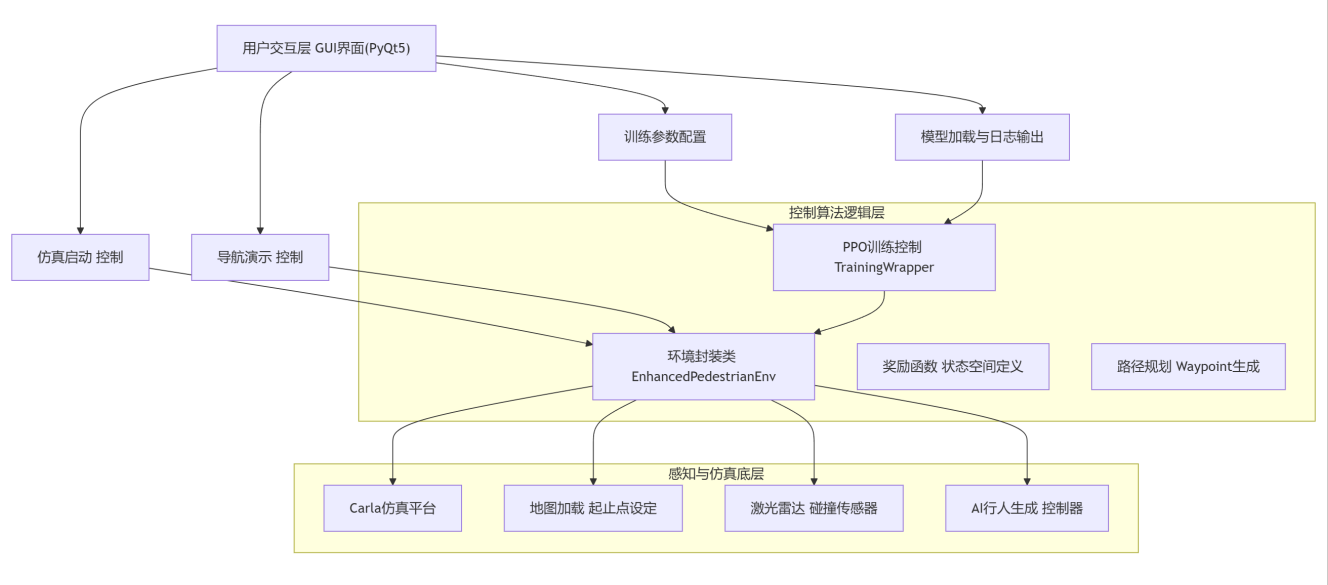
\includegraphics[width=1\textwidth]{images/nav_system_architecture.png}
    \caption{系统总体结构图}
    \label{fig:system-architecture}
\end{figure}

\textbf{底层感知层}:该层负责Carla仿真平台的连接和初始化传感器,通过Python的API生成行人生成路径采样、目标点采样和路径采样的过程,激光雷达、碰撞传感器实时扫描环境。

\textbf{中间控制逻辑层}:该层为系统的内核逻辑层,即定义强化学习环境、奖励函数体系、PPO训练模型等。在学习的回合中,环境返回动作的奖励,并进行状态更新;在推理过程中,策略网络在状态上推理,并进行状态更新。

\textbf{用户交互层}:基于PyQt5构建GUI(v1.4版本以优化为基于PyQt6),用户可视化设置参数(如训练步数、目标点、导航模式),并实时查看导航状态、训练进度、路径规划图等。界面还支持导入模型与输出路径记录。如图 \ref{fig:location},当用户点击显示可生成行人位置时,地图上便会出现所有可以用来生成行人位置的地方,以方便用户进行初始地点和目标地点的选取。

\begin{figure}[H]
	\centering
	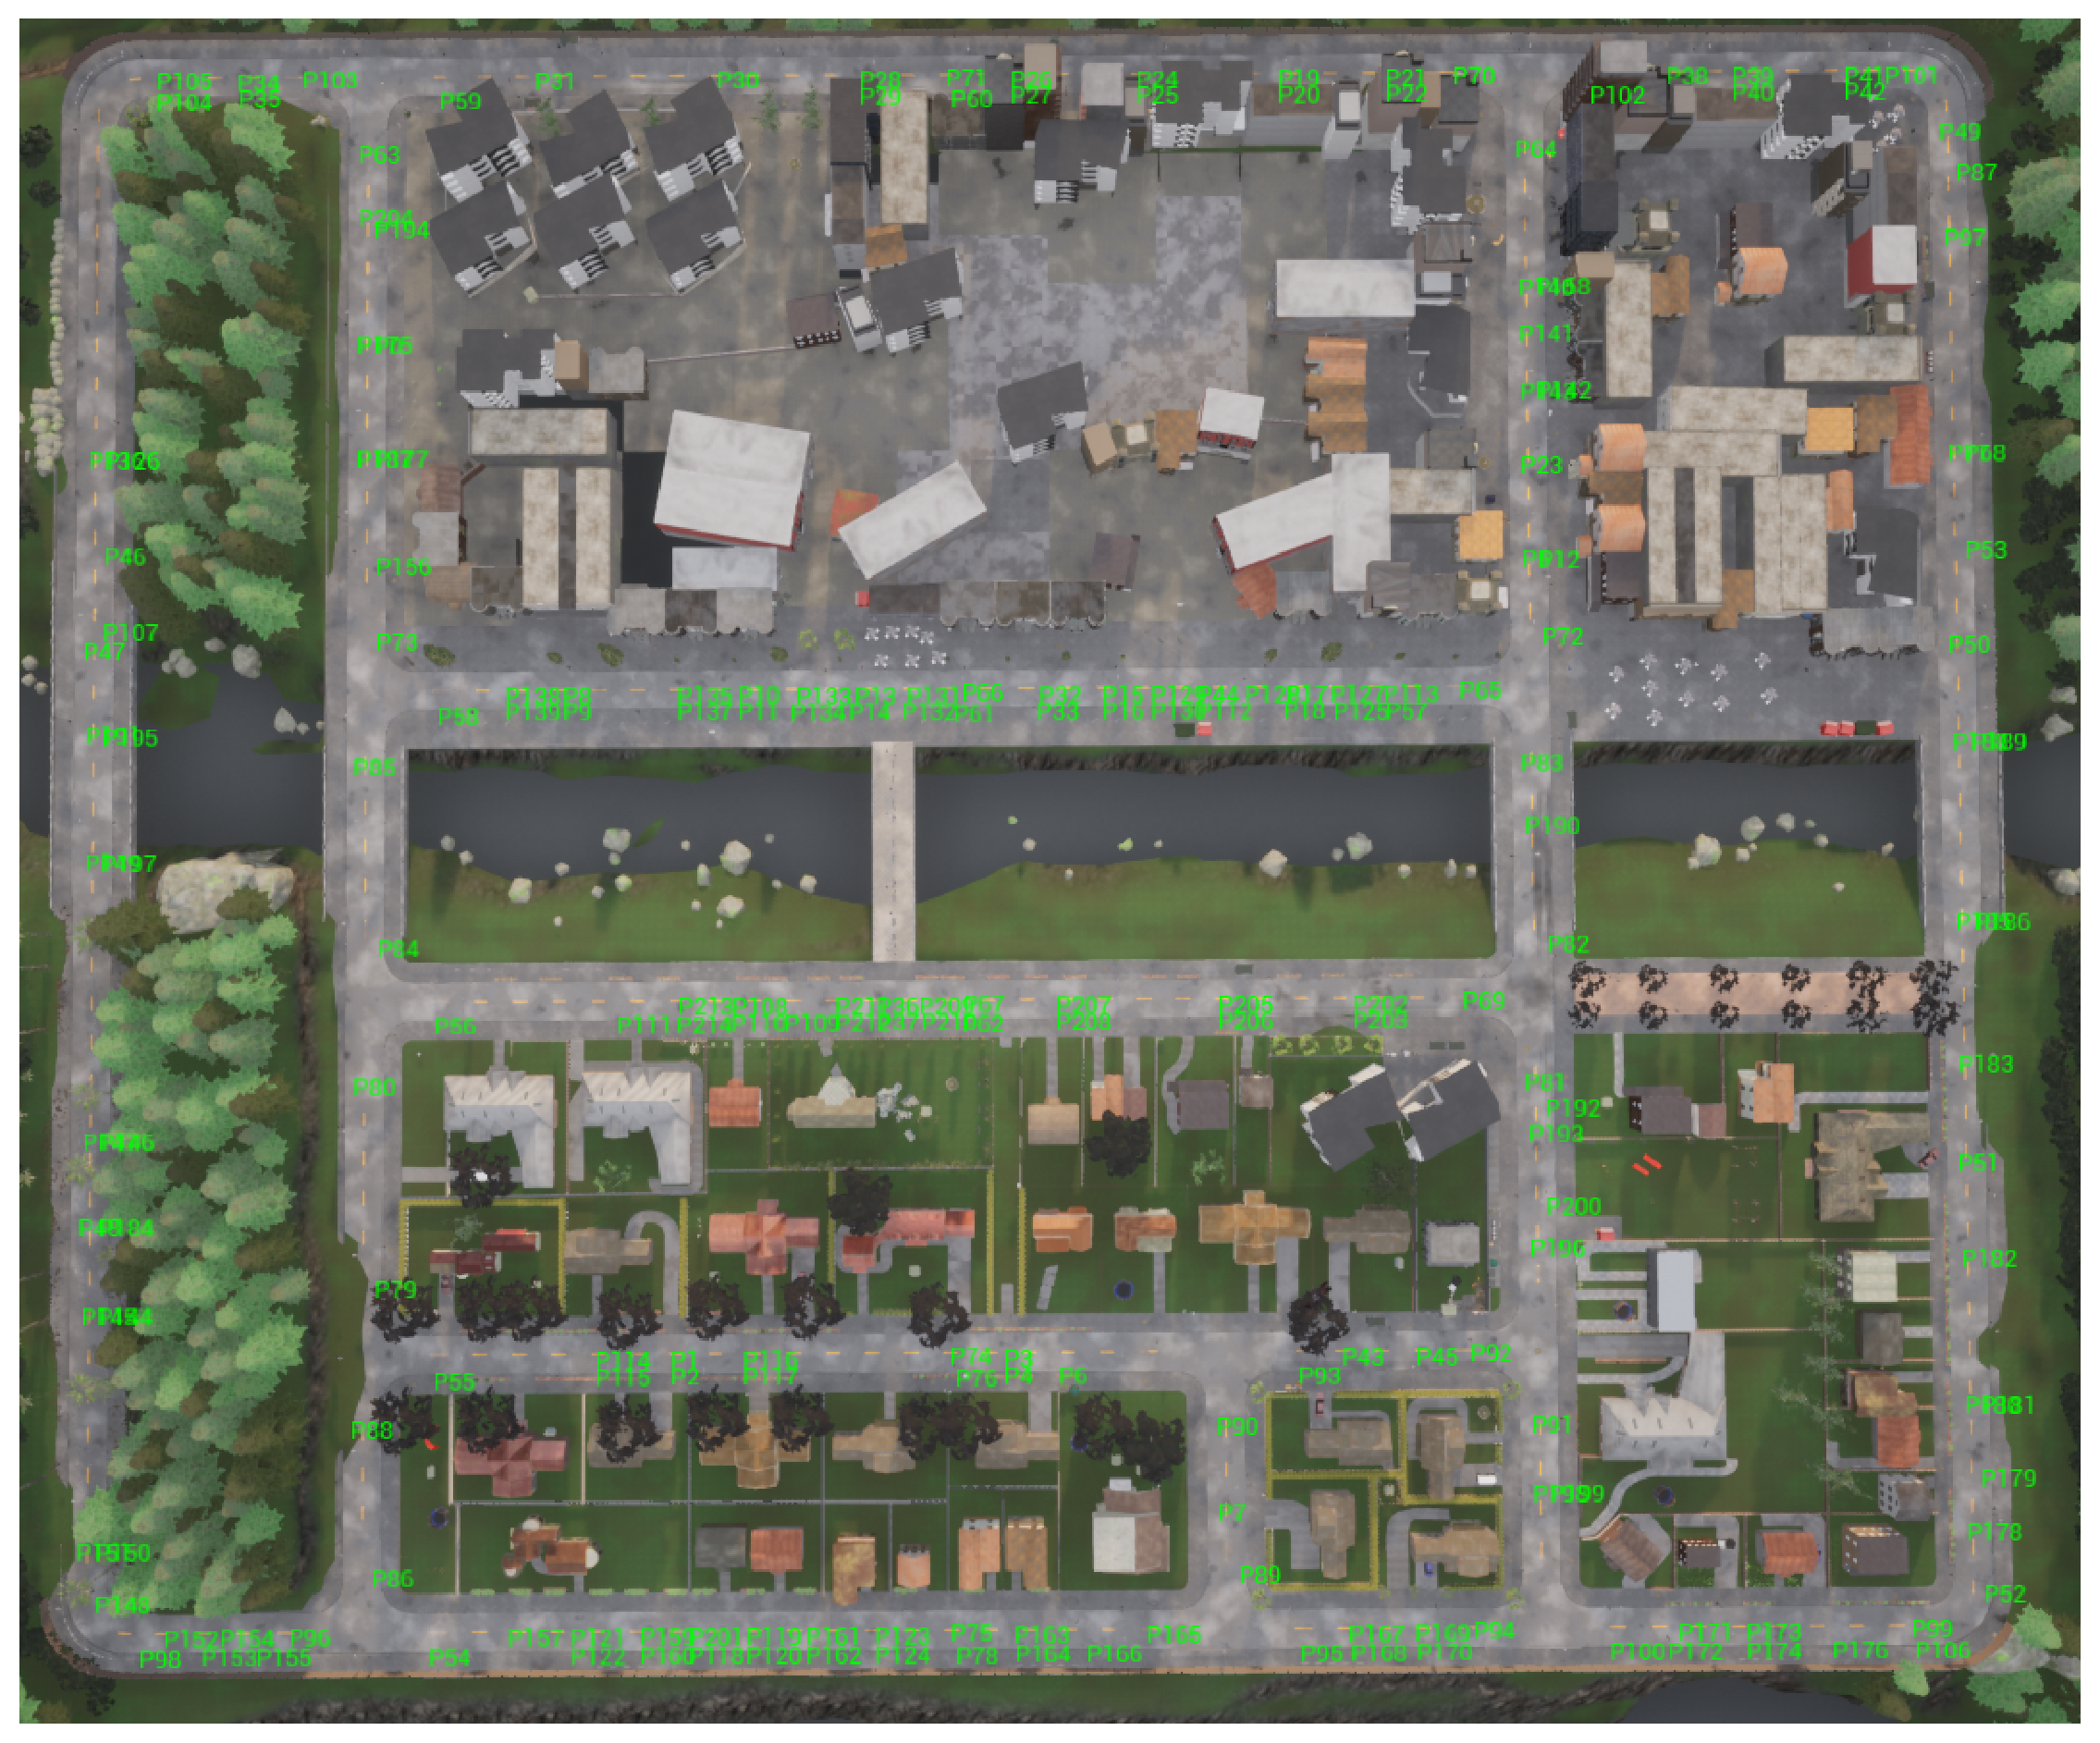
\includegraphics[width=1\textwidth]{images/location_point.pdf}
	\caption{可生成行人位置示意图}
	\label{fig:location}
\end{figure}
	
\section{模型训练奖励函数设计}
	
强化学习任务中奖励函数设计至关重要,在行人导航系统中其直接影响智能体决策行为,合理设计奖励函数是实现高效稳定导航的关键,以下为本系统奖励函数的设计思想与实现细节:
	
\subsection{目标达成奖励}
目标达成奖励的目的是鼓励行人尽快接近目标,并在接近时给出更高的奖励。通过根据目标距离的变化量来调整奖励,确保模型能够学习到快速、有效的路径规划。
	
\begin{equation}
R_{\text{target}} =
\begin{cases}
1000 \cdot \mathbb{X}(d_{\text{target}}<3) & \text{终止条件} \\
\Delta d \times 50 \times \left(1 - \frac{d_{\text{target}}}{100}\right) & \text{常规状态}
\end{cases}
\end{equation}
其中:
\begin{itemize}
	\item \( \Delta d = d_{\text{prev}} - d_{\text{target}} \) 表示单步距离变化量
	\item 动态系数强化近距离奖励:\( d_{\text{target}} \) 在 \([0, 100]\) 范围内时,系数从1.0线性衰减至0.0
\end{itemize}
	
\subsection{路径跟踪奖励}
路径跟踪奖励旨在鼓励行人沿着预定的路径行进。通过计算行人与路径的横向偏差来调整奖励,确保行人尽量沿着正确的路线行走。
	
\begin{equation}
R_{\text{path}} =
\begin{cases}
1.5 \cdot \left(1 - \frac{\Delta_{\text{dev}}}{2}\right) & \Delta_{\text{dev}} \leq 2\ \text{m} \\
-1.0 & \Delta_{\text{dev}} > 2\ \text{m}
\end{cases}
\end{equation}
其中:
\begin{itemize}
	\item \( \Delta_{\text{dev}} = \left\| \vec{p}_{\text{current}} \times \vec{v}_{\text{forward}} \right\| / \left\| \vec{v}_{\text{forward}} \right\| \) 为路径偏差的计算方法。
\end{itemize}
	
\subsection{安全避障机制}
安全避障机制的目的是通过惩罚碰撞事件和危险距离来确保行人安全,避免与障碍物发生碰撞。
	
\begin{equation}
R_{\text{safety}} =
\begin{cases}
-500 \cdot \mathbb{X}_{\text{collision}} & \text{碰撞事件} \\
-\dfrac{0.5}{d_{\text{obs}} + 0.5} & d_{\text{obs}} \leq 2\ \text{m} \\
-(v_{\text{prev}} - v_{\text{curr}}) & \Delta v > 1\ \text{m/s}
\end{cases}
\end{equation}
其中:
\begin{itemize}
	\item \( \mathbb{X}_{\text{collision}} \) 表示碰撞事件,碰撞时给予-500的惩罚。
	\item \( d_{\text{obs}} \) 为障碍物的最小距离,若小于2米,则按距离反比例惩罚。
	\item \( \Delta v = v_{\text{prev}} - v_{\text{curr}} \) 为速度变化,若速度骤降超过1米每秒,则给予惩罚。
\end{itemize}
	
\subsection{运动模式优化}
运动模式优化的目的是确保行人的速度保持在合适范围内。通过设定不同速度区间的奖励,鼓励行人在不同距离的情境下选择合适的速度。
	
\begin{equation}
R_{\text{motion}} =
\begin{cases}
0.2 & \text{低速合规}(0.3 \leq v \leq 1.0)\ \cap\ d_{\text{target}} < 5\ \text{m} \\
0.1 & \text{中速合规}(0.5 \leq v \leq 1.5) \\
-0.2(v-1.0) & \text{超速状态}(v > 1.0)\ \cap\ d_{\text{target}} < 5\ \text{m}
\end{cases}
\end{equation}
	
\subsection{时间效率惩罚}
时间效率惩罚的目的是防止模型做出过多无效的移动或徘徊,鼓励快速完成任务。
	
\begin{equation}
R_{\text{time}} = -0.01 \cdot t_{\text{step}}
\end{equation}
其中:
\begin{itemize}
	\item 每一步都会施加一个固定的时间惩罚,以鼓励高效的路径规划。
\end{itemize}
	
\subsection{终止条件奖励}
终止条件奖励的目的是当模型达到目标位置时给予额外奖励,或者在碰撞时进行终止。
	
\begin{equation}
R_{\text{terminal}} =
\begin{cases}
+1000 \cdot \mathbb{X}(d_{\text{target}} < 2\ \text{m}\ \cap\ \theta_{\text{error}} < 45^\circ) & \text{精确到达} \\
-500 \cdot \mathbb{X}_{\text{collision}} & \text{碰撞终止}
\end{cases}
\end{equation}
其中:
\begin{itemize}
	\item \( \theta_{\text{error}} = \left| \arctan\left(\frac{-\Delta y}{\Delta x}\right) - \theta_{\text{current}} \right| \) 表示当前朝向与目标方向之间的角度偏差。
	\item 双重终止条件确保目标点朝向正确性。
\end{itemize}
	
\subsection{综合奖励架构}
综合奖励架构的目的是将各个独立的奖励信号进行加权求和,形成一个最终的奖励值。这可以确保模型在考虑多个目标时进行平衡。
	
\begin{equation}
R_{\text{total}} = R_{\text{target}} + R_{\text{path}} + R_{\text{safety}} + R_{\text{motion}} + R_{\text{time}} + R_{\text{terminal}}
\end{equation}

该奖励函数由\( R_{\text{target}} \) 、\( R_{\text{path}} \) 、\( R_{\text{safety}} \) 、\( R_{\text{motion}} \)、 \( R_{\text{time}} \) 、\( R_{\text{terminal}} \)等部分构成,其中 \( R_{\text{target}} \) 为目标达成奖励旨在激励智能体尽快接近导航终点;\( R_{\text{path}} \) 为路径跟踪奖励鼓励智能体沿预设路径平稳前进;\( R_{\text{safety}} \) 为安全奖励用于约束行人规避碰撞与危险区域;\( R_{\text{motion}} \) 为运动模式奖励通过引导合理速度与姿态优化行进行为;\( R_{\text{time}} \) 为时间效率惩罚用于约束过慢行为提升总体路径效率;\( R_{\text{terminal}} \) 为终止条件奖励用于在任务完成时给予最终正向激励。

\subsection{具体实现}
通过上述奖励函数的设计,使行人导航系统实现智能体在环境中的避障,快速到达目标,对自身的行动决策方案不断优化来寻找最优路径。本节通过环境中具体场景的设定和相应传感器的帮助完成导航,如:观测空间耦合,动态奖励系数计算,路径可视化等。
	
本系统的路径规划与训练环境具有多项关键特征。观测空间采用12维特征向量形式,集成了局部路径点坐标 \(x_{\text{wp}}, y_{\text{wp}}\)、障碍物距离 \(d_{\text{obs}}\) 等状态信息,增强了状态表示能力与感知精度。奖励函数中引入目标距离因子 \(1 - \frac{d}{100}\),实现奖励强度随导航进展自适应变化,提升训练灵敏度与稳定性。安全机制设计为分层结构,依次包括碰撞检测模块、障碍物距离判断与速度变化分析,三者构成对复杂环境中行人行为的全方位保护。路径点通过Carla平台调试接口实时渲染与可视化,为模型训练提供可观测的反馈支撑。
	
\section{路径规划与避障设计}
	
为了实现行人从起点自主导航至终点的位置,本系统基于 Carla 仿真平台的人行道地图信息实现了路径规划模块,并结合激光雷达传感器与碰撞检测机制设计了避障逻辑,从而使得训练与推理过程具备高度的真实交互性与安全性。
	
\subsection{路径规划机制}

\subsubsection{Waypoint路径规划}
	
本系统的v1.2和v1.3版本的路径规划机制采用 Carla 提供的人行道导航信息,基于其地图 Waypoint 系统进行路径规划。行人生成后,通过设定的起点和终点位置,路径规划模块使用以下流程自动生成一条可通行的人行道路径:

首先将生成的起点与目标位置映射为距离最近的人行道类型(Sidewalk)Waypoint,确保路径生成遵循场景中的通行规则。路径拓展采用基于距离阈值的前向搜索策略,从起点出发调用 \texttt{waypoint.next(distance)} 方法连续生成多个路径点,直到所生成路径接近目标位置为止。所有路径点以 \texttt{planned\_waypoints} 列表形式保存,并通过Carla平台的Debug模块以箭头形式绘制于场景中,提供路径可视化支持与调试依据。

该路径规划策略具备多方面优势,能够确保路径始终沿合法人行道生成以避免穿越非通行区域并符合交通规则与仿真约束,同时路径生成精度可通过调整采样分辨率进一步优化以满足不同任务场景精细化需求,遇到异常或失败情况时系统触发回退或重试逻辑以提升整体鲁棒性与容错能力。

\begin{figure}[H]
	\centering
	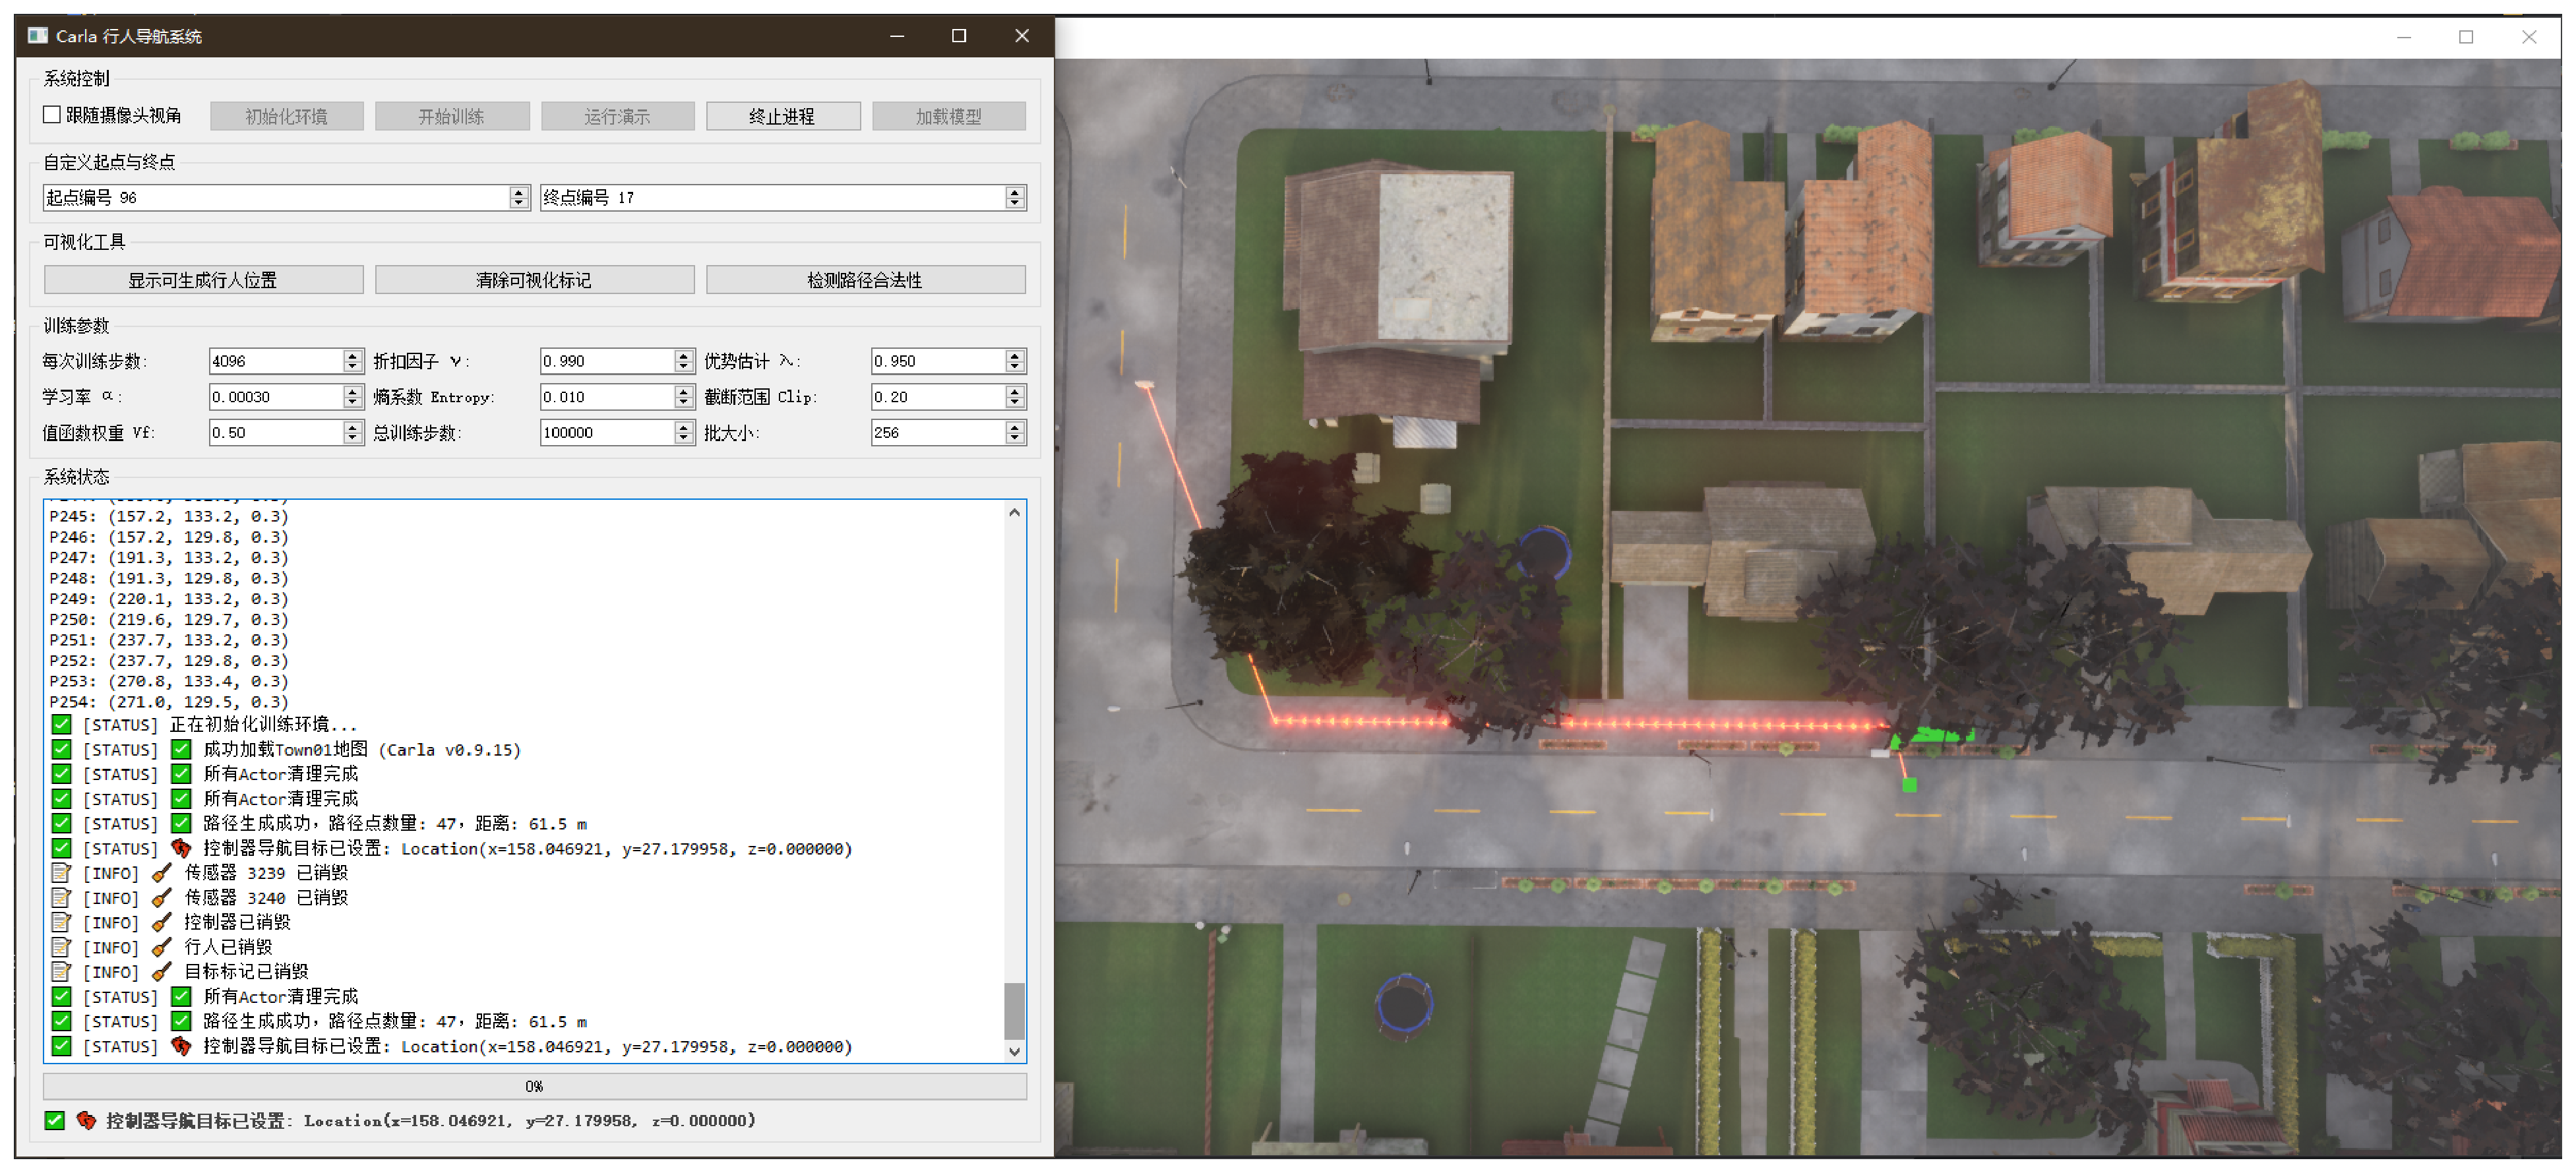
\includegraphics[width=1\textwidth]{images/path_waypoint1.pdf}
	\caption{旧版红色箭头路径示意图}
	\label{fig:way1}
\end{figure}

如图 \ref{fig:way1}所示地图上生成的红色箭头为路径规划标记,因生成箭头限制在 200 个以内且采用强制到达终点设计导致导航路径显得较为生硬,这些可通过后期硬件提升和版本优化改善。

\subsubsection{A*启发式搜索算法}

A*算法是一种启发式搜索算法,用于在加权图中高效寻找两点间最短路径。其核心通过综合评估路径代价优化搜索方向,特征如下:

\paragraph{算法原理:}
\begin{enumerate}
    \item \textbf{代价函数}:算法以总代价函数作为路径评估依据,形式为
    \[
    f(n) = g(n) + h(n)
    \]
    其中,$g(n)$表示从起点到当前节点$n$的累计实际代价,$h(n)$表示从节点$n$到目标位置的估算代价,常以欧氏距离进行计算。

    \item \textbf{数据结构}:算法维护两个核心节点集合。开放列表按照总代价$f(n)$排序,用于存放尚未扩展的节点;封闭列表用于记录已被探索的节点,从而避免重复搜索。

    \item \textbf{搜索流程}:将起点纳入开放列表后,反复选取总代价最小的节点进行处理,若该节点为目标位置则开始路径回溯,否则扩展其所有邻接节点,更新这些节点的总代价并调整开放与封闭列表。
\end{enumerate}

\paragraph{关键性质:}

\begin{enumerate}
    \item \textbf{可接受性}:启发函数必须满足估算代价不超过最短实际代价
    \[
    h(n) \leq h^*(n)
    \]
    其中$h^*(n)$为从节点$n$到目标的真实最短代价,此条件保证算法能够得到最优路径。

    \item \textbf{一致性}:若启发函数满足
    \[
    h(n) \leq c(n, n') + h(n')
    \]
    其中$c(n, n')$为节点$n$到其邻接节点$n'$的移动代价,则算法在搜索过程中不会重复扩展任何节点,提升效率。
\end{enumerate}

\paragraph{代码实现:}
\begin{enumerate}
    \item \textbf{启发函数选择}:使用欧氏距离$h(n) = \|n_{\text{current}} - n_{\text{target}}\|_2$,满足可接受性
    \item \textbf{路径搜索}:调用NetworkX库函数\texttt{nx.astar\_path},输入图结构、起点、终点及启发函数
    \item \textbf{异常处理}:路径搜索失败时记录错误日志,检查起点终点是否位于同一连通子图
\end{enumerate}
	
\begin{figure}[H]
	\centering
	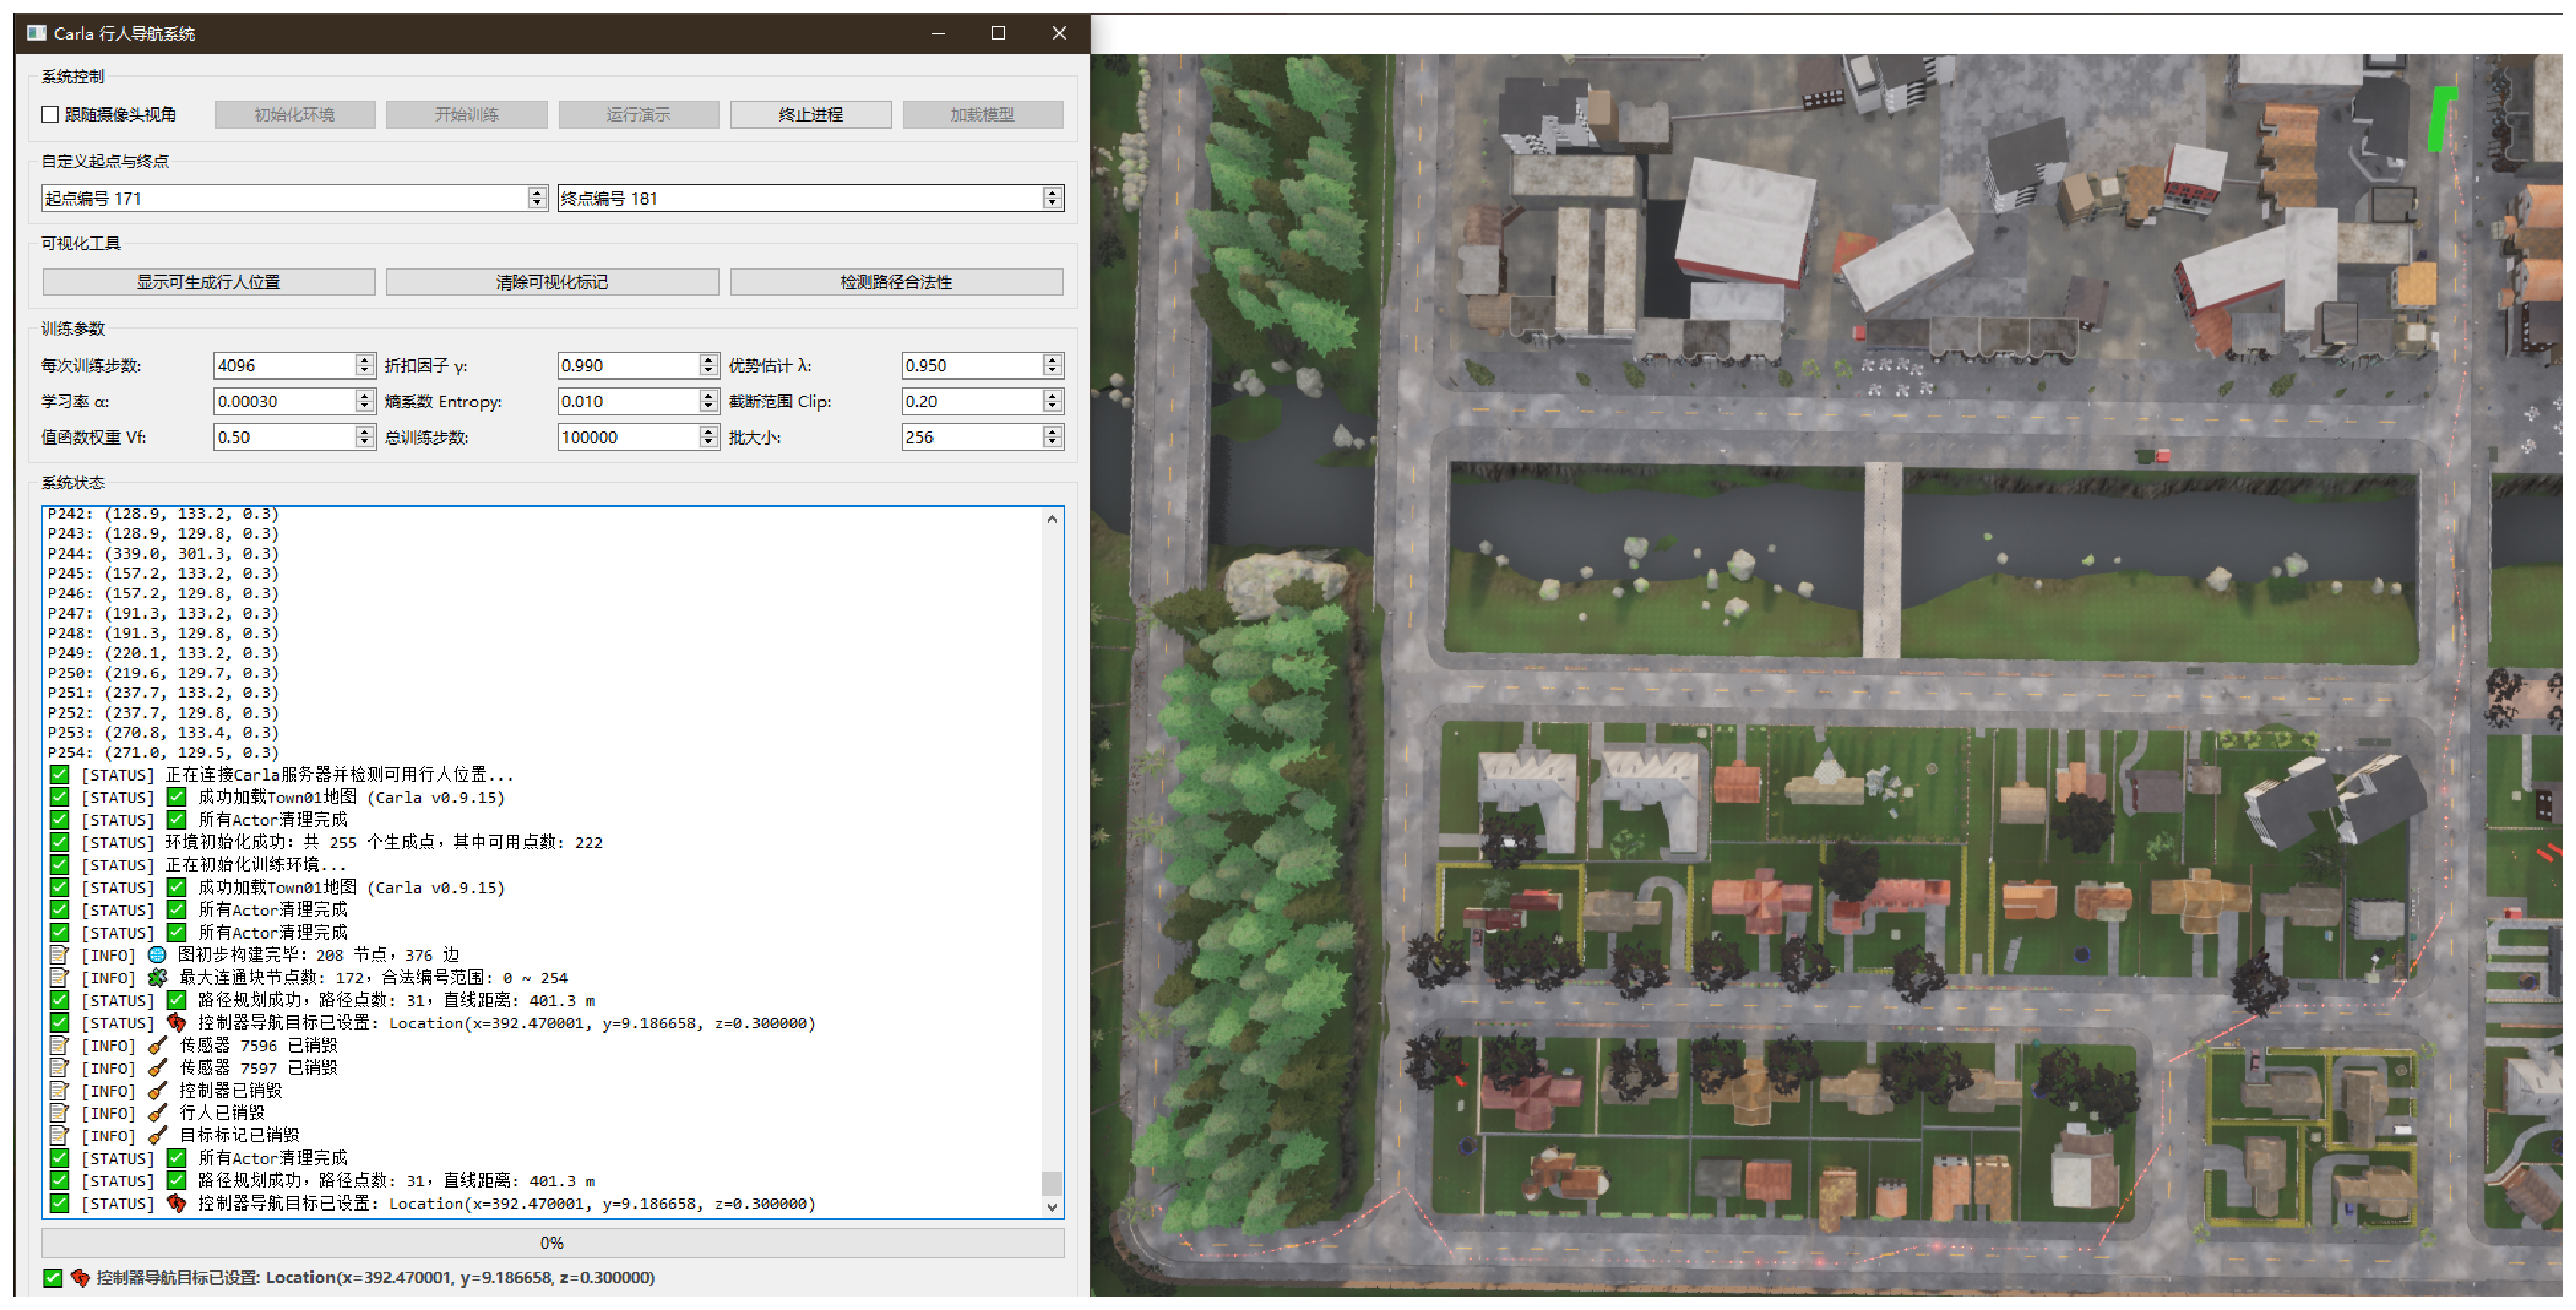
\includegraphics[width=1\textwidth]{images/path_waypoint2.pdf}
	\caption{新版红色箭头路径示意图}
	\label{fig:way2}
\end{figure}

如图 \ref{fig:way2}所示的路径规划机制基于预先生成的静态可行走点构建导航图,通过A*算法实现路径搜索与优化。具体流程如下:可行走点数据从CSV文件加载,每个点包含坐标与唯一索引。利用k近邻方法将每个点与其最近的6个相邻点连接形成无向图,边权重为欧氏距离。通过提取最大连通子图确保路径可达性,避免无效路径生成。A*算法以欧氏距离为启发函数搜索起点至终点的最短路径,调用NetworkX库实现路径节点序列生成。路径需满足长度约束(20-200个点)且起点终点索引必须属于最大连通图合法编号集合。规划结果转换为虚拟路径点序列,行人控制器根据路径点动态设定目标位置。激光雷达实时检测障碍物距离,结合路径偏差计算与强化学习奖励机制调整行人转向及速度。路径可视化通过Carla调试工具实现,红色箭头标记规划路径,绿色点显示行人轨迹,起点与终点分别标注为“Start”和“Goal”,由于此标记为限时显示故此图中未标出,但可以看到一个绿色小点即为初始行人生成点。系统通过合法性检测功能验证路径对有效性,确保训练与演示的可行性。代码核心模块包含图构建、A*搜索、路径更新及控制逻辑,其特点为静态环境假设、障碍物实时避障与多维度可视化支持。图 \ref{fig:perspective1}和图\ref{fig:perspective2}展示了其他视角下路径规划出来的红色箭头,便于用户更直观的理解。

\begin{figure}[H]
	\centering
	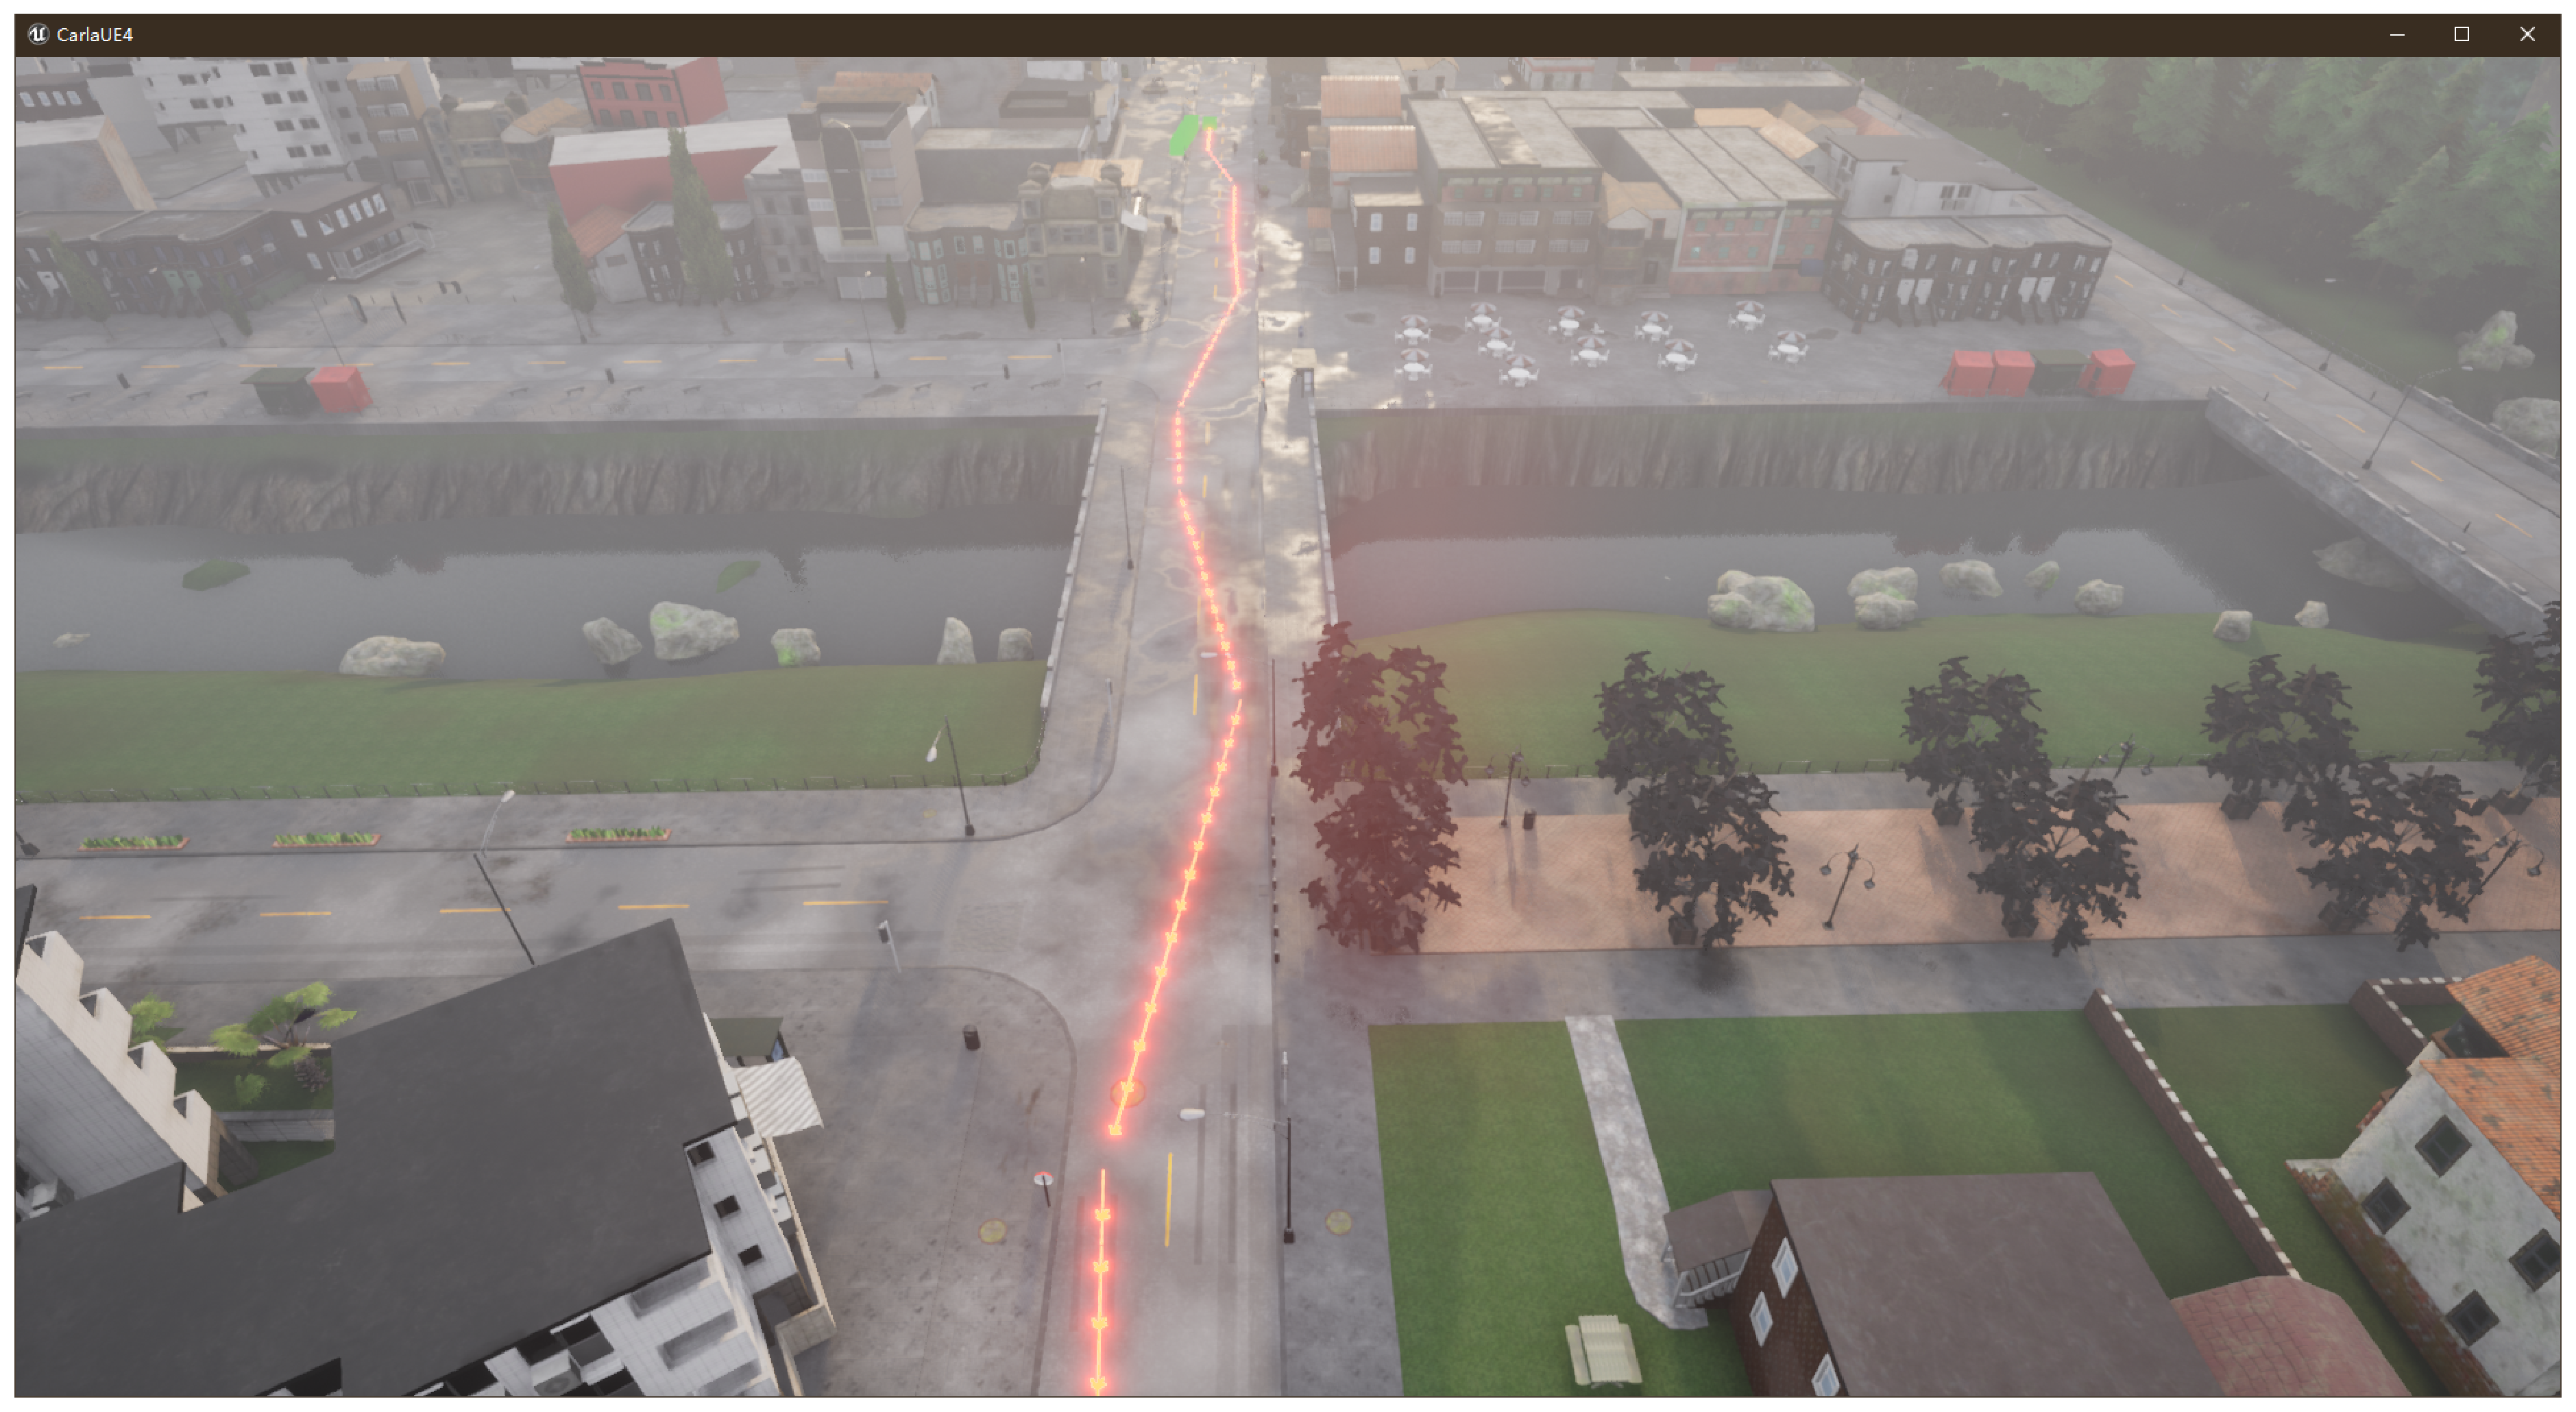
\includegraphics[width=1\textwidth]{images/nav_perspective1.pdf}
	\caption{起点视角}
	\label{fig:perspective1}
\end{figure}

\begin{figure}[H]
	\centering
	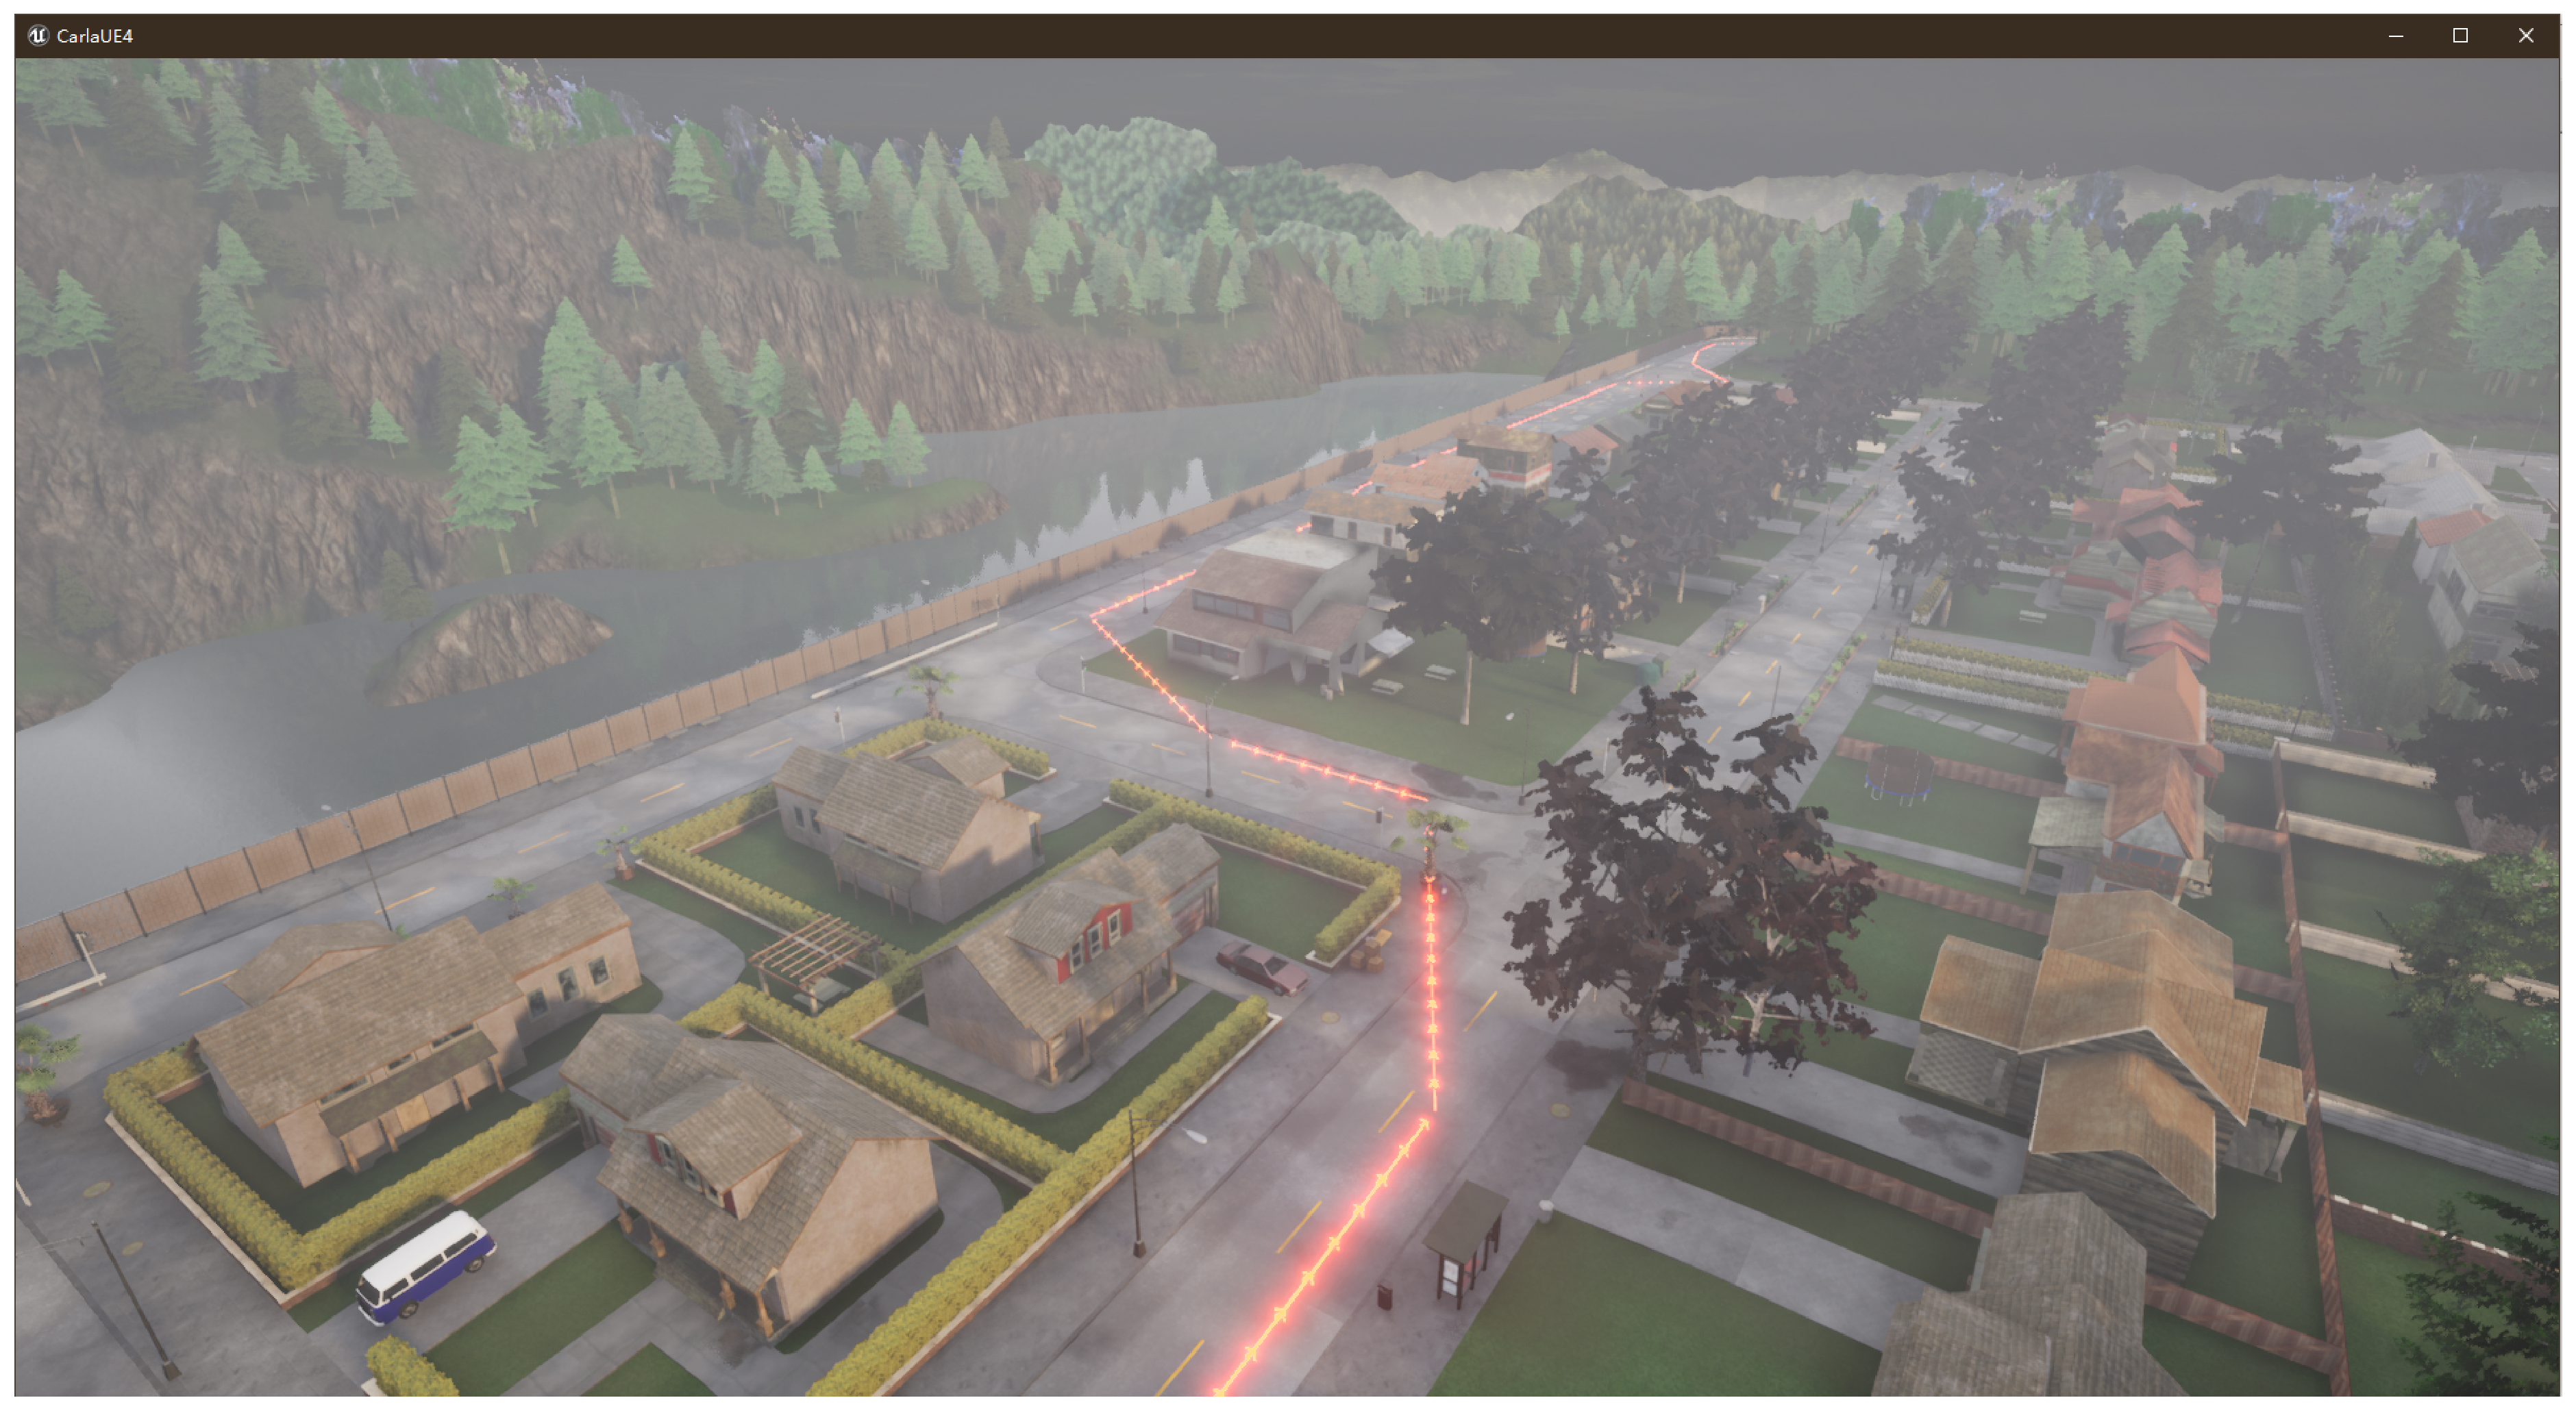
\includegraphics[width=1\textwidth]{images/nav_perspective2.pdf}
	\caption{终点视角}
	\label{fig:perspective}
\end{figure}
	
\subsubsection{避障与动态反应机制}

避障模块主要是根据激光雷达传感器从 Carla 平台实时返回的回传点云信息进行避障响应,在每次获取到的点云数据中寻找离障碍物最近点的最小值\texttt{min\_obstacle\_d\\istance},作为当前避障初始化值,若小于 2.0m 则速度减小,将行人的当前避障初始化值减小至小于 0.8m/s,降低行人的碰撞概率。在奖励函数中增加避障的惩罚,如果行人离障碍物太近且速度较快的话,扣减一定的奖励值,从奖励角度避免智能体采取危险动作。同时,如果检测到碰撞传感器,则立即退止出小节,对智能体进行大惩罚(-500),增加对碰撞信息的反馈权重。

该机制将传感器、速度控制器、奖励函数调整三个部分算法结合起来,构成一个完整的避障控制算法。Agent在训练中动态复杂的环境中学习如何规划路径,在避障和路径规划之间寻找一个平衡点,使路径规划更安全稳定。
	
\subsection{路径规划与避障的协同工作}
	
路径规划模块和避障模块之间是紧密相连的,为了保证路径的安全可靠,行人在沿着规划路径行走的同时,不断在路径中利用激光雷达和碰撞传感器等进行障碍物探测,遇到阻挡物时进行避让处理,避免碰撞,避免偏离规划路径,并在进行避障处理后,路径规划模块及时重新寻找最优路径并继续向着目标路径行走,确保行人在复杂的路径环境中向着目标方向行走,安全有效的完成路径任务。

\section{本章小结}

本章介绍了行人导航系统的设计方案,以构建具备环境感知、路径规划及避障功能的行人智慧导航应用平台作为系统最终目标,对复杂城市场景中的行人导航应用系统进行场景化设计。首先明确了系统实现的快速路径规划、避障感知与避障控制、交互与可视化等主要功能,从非功能性、功能性角度进行系统需求分析;设计感知、控制与交互三部分构成的三层系统模型,对系统各部分进行分工与相互关系说明;设计奖励函数作为强化学习的关键内容,并从实现目标达成、路径追踪、安全规划与效率规划等子问题出发,提升行人导航学习的实时收敛效率;对行人路径规划模型、避障控制策略与训练环境设置等核心实现部分进行描述,为之后实验分析及模型效果评估提供系统平台。

	
